\subsection{Cubrimientos}
El estudio mediante cubrimientos se basa en la idea de estudiar los
caminos de un espacio base \((X, x_0)\) viendo como lucen estos en
un espacio de cubrimientos \((\tilde X, \tilde x_0)\) a través de la
inversa de una función sobreyectiva \(p : \left( \tilde X, \tilde x_0
\right) \to \left( X, x_0\right)\). Se definirán estos conceptos formalmente
\begin{definicion} \label{def:cubierta}
Sea \(p : \tilde{X} \to X\) una función continua sobreyectiva. El
abierto \(U \subseteq X\) se dice \textbf{cubierto} por \(p\)
si existe \(\{V_\alpha\}_{\alpha \in \Lambda},\ \Lambda \subseteq
\mathbb N\) tal que
\[ p^{-1} (U) = \bigcup_{\alpha \in \Lambda} V_\alpha \]
Donde \(\{V_\alpha\}\) es una familia disjunta de abiertos, tal que
\(\forall \alpha \in \Lambda\) la restriccion \( p \mid_{\alpha}\) es
homeomorfa sobre \(U\). Si para todo \(x \in X\) existe una vecindad
\(U\) que cumpla lo anterior, se dirá que \(\tilde{X}\) es un
\textbf{espacio cubrimiento} de \(X\) y el par \((p,\tilde X)\) denota
el cubrimiento para \(X\).
\end{definicion}

\begin{ejemplo}[Cubrimiento de \(S^1\) por \( \begin{bmatrix} 0, 10
\pi \end{bmatrix} \) con \( 0 \sim 10 \pi \)] \label{ej:10pi}
  Pensamos en \(S^1\) como el intervalo \([0, 2 \pi]\) enrollado sobre
  si mismo mediante la identificacion \(0 \sim 2 \pi\). Podemos imaginar
  un cubrimiento de este como cualquier intervalo con los extremos
  identificados que de al menos una vuelta completa a \([0, 2 \pi]\).
  \begin{figure}[h]
    \centering 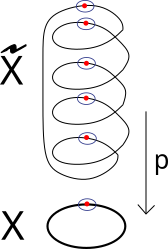
\includegraphics[scale=0.5]{./imagenes/spring.png}
  \end{figure}
  Ciertamente el intervalo \([0, 10 \pi]\) con \(0 \sim 10 \pi\) cumple
  el requisito, con el cubrimiento dado por
  \begin{align*}
    p : [0, 10 \pi] / _{(0 \sim 10\pi )} &\longrightarrow [0, 2 \pi] / _{(0 \sim 2\pi )} \\
    t &\longmapsto \mathrm t \mod 2 \pi
  \end{align*}
\end{ejemplo}
El diagrama anterior da una idea de la forma de general los espacios
cubrimientos \(\tilde X\), estos lucen como iteraciones del espacio base
\(X\). Por otro lado, sea \(x_0 \in S^1\) el punto rojo del diagrama, se
tiene la siguiente definicion auxiliad
\begin{definicion}[Fibra]
El conjunto discreto dado por \(p^{-1} (x_0)\) es conocido como una
\emph{fibra} de \(x_0\).
\end{definicion}
\noindent Una invariante interesante de este es que la cardinalidad de
cualquier fibra es la misma para todos los puntos.

\begin{ejemplo}[Cubrimiento de toro]
  En el ejemplo \ref{ej:toro-presentacion} se trabajo con la
  presentación de toro como espacio cociente de \([0,1]^2\). Siguiendo
  la idea del ejemplo anterior, podemos obtener un cubrimiento de esta
  presentación mediante el siguiente diagrama.
  \begin{figure}[h]
    \centering 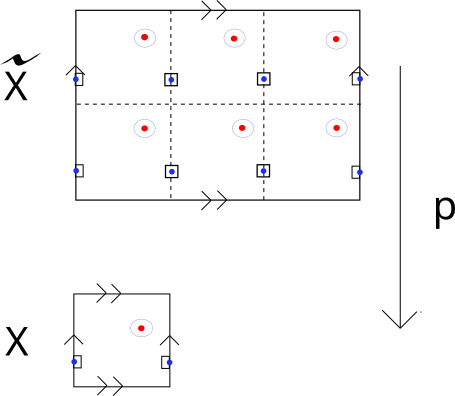
\includegraphics[scale=0.5]{./imagenes/toro-cubrimiento.png}
  \end{figure}
\end{ejemplo}

\begin{ejemplo}[Cubrimiento: \(\Re\) sobre \(S^1\)]
Para \(S^1\) el mapeo
\begin{align*}
  p : \Re &\longrightarrow S^1 \\
  t &\longmapsto e^{2 \pi \imath t}
\end{align*}
es claramente
sobreyectivo y continuo. Escogiendo dos abiertos ejemplares como \(U =
S^1 - \{(1,0)\}\) y \(V = S^1 - \{(-1,0)\}\), es claro que
\[
    p^{-1} (U) = \bigcup_{n \in \mathbb Z} (n, n+1)
    \qquad p^{-1} (V) = \bigcup_{n \in \mathbb Z} (n - \frac 1 2, n + \frac 1
    2 )
\]
Donde estas familias de conjuntos son disjuntos y restringidos a cada
uno se tiene la inyectividad requerida.
\end{ejemplo}

A priori el cubrimiento es independiente de los caminos que tengamos
en \(X\), queremos ver si podemos reflejar la información importante de
los caminos de \(X\) sobre \(\tilde{X}\);
\begin{figure}[h]
  \centering
  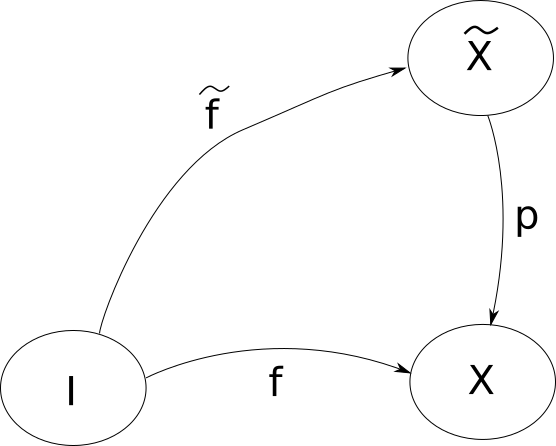
\includegraphics[scale=0.3]{./imagenes/lifting-path.png}
\end{figure}
es decir, para todo arco \(f : I \to X\), construiremos \(\tilde f : I
\to \tilde X\) el cual cumpla \(p \circ \tilde f = f \), donde \(\tilde
f\) sera nuestro representante en el espacio cubrimiento de este
camino. Veremos también que bajo ciertas hipótesis, este \(\tilde f\)
es único y refleja información homotopica. Para esto necesitamos
desarrollar algunos teoremas previos.
\begin{lema}[Numero de Lebesgue] \label{thm:lebesgue-number-lema}
  Sea \(\mathcal A\) un cubrimiento del espacio métrico \((X,d)\). Si
  \(X\) es compacto, entonces existe \(\delta > 0\) tal que para todo
  subconjunto de \(X\) teniendo diámetro menor que \(\delta\), existe un
  elemento de \(\mathcal A\) conteniéndolo.
\end{lema}
\begin{proof}
  Supongamos que \(X \not \in \mathcal A\), pues si no trivialmente el
  teorema se cumple \(\forall \delta > 0\). Por compacidad de \(X\)
  existe una colección \(\{A_1,\dotsc,A_n\} \subset \mathcal A\) que
  cubre a \(X\), definamos a los conjuntos \(C_i = X - A_i,\ \forall i
  \in [1,n]\) y a la función \(f : X \to \Re\) definida por
  \[ f(x) := \frac 1 n \sum_{i=1}^{n} d(x, C_i) \]
  i.e. la distancia promedio de \(x\) a \(C_i\). Notemos que \(\forall x
  \in X,\ f(x) > 0\), pues para \(x \in A_i \subseteq X\), por ser
  \(A_i\) un abierto, existe \(\epsilon > 0\) tal que \(B(x,\epsilon)
  \subset A_i\) y por tanto \(d(x, C_i) \geq \epsilon\) que implica \(
  f(x) \geq \frac \epsilon n > 0\).

  Por otro lado \(f\) es una función continua sobre \(X\) un espacio
  compacto, por lo tanto alcanza un mínimo; a este le denotaremos como
  nuestro \(\min_X f \coloneqq \delta \).

  Probaremos que este \(\delta\) cumple el requerimiento. Sea \(B
  \subset X\) subconjunto abierto de diámetro menor que \(\delta\), sea
  \(x \in B\) arbitrario. Escojamos el conjunto \(C_m\) como
  \[ C_m := \max_{i \in [1,n]} d(x, C_i) \]
  Dado que
  \[\delta \leq f(x) \leq d(x, C_m) \]
  Esto nos dice que dado \(\delta \leq d(x, C_m)\), existe una vecindad
  de al menos diámetro \(\delta\) que contiene a \(x\) en \(X - C_m = A_m\).
\end{proof}
\begin{definicion}[Levantamiento de \(f\)]
  Sea \(p : \tilde X \to X\) un mapeo. Si \(f : W \to X\) es un mapeo
  continuo, un levantamiento de \(f\) es una función \(\tilde f : W \to
  \tilde X\) tal que \(p \circ \tilde f = f\).
\end{definicion}
Ver que la definición es mucho mas general que lo que pedíamos al
diagrama. Usualmente \(W = [0,1]\) pues estudiaremos los caminos sobre
\(X\). Veremos a continuación teoremas de como se reflejan los caminos
y las homotopías en el espacio cubrimiento de \(X\).
\begin{teorema}[Levantamiento de caminos] \label{thm:lifting-theorem}
  Sea \(p : \tilde X \to X\) un cubrimiento y \(x_0 \in X\). Fijemos
  algún \(\tilde x _0 \in \tilde X\) tal que \(p(\tilde x _0) = x_0 \).
  Para cualquier camino \(f : [0,1] \to X\) que comience en \(x_0\), existe
  un único camino levantamiento \(\tilde f : [0,1] \to \tilde X\) tal que
  \(\tilde f (0) = \tilde x _0\)
\end{teorema}
\begin{proof}
  Para todo punto de \(x \in X\), existe una vecindad de este \(U_x\)
  que es cubierta (definicion \ref{def:cubierta}). Por tanto
  \[ X \subseteq \bigcup_{x \in X} U_x\]
  con \(U_x\) siendo las vecindades cubiertas para cada \(x\). De lo
  anterior, se obtiene la siguiente inclusion
  \[ [0,1] = f^{-1} \left( X \right) \subseteq f^{-1} \left( \bigcup_{x
    \in X} U_x \right) \]
  Por el Teorema \ref{thm:lebesgue-number-lema}, podemos elegir
  \(s_0,\dotsc,s_n \in [0,1]\) tal que para todo \(i \in \{0,1 \dotsc,
  n-1\}\), exista \(U_x\) tal que
  \[f \left( [s_i, s_{i+1}] \right) \subset U_x \]
  Con esto, definiremos \(\tilde f\) inductivamente.

  Primero declaremos \(\tilde f (0) = \tilde x _0\). Luego, suponiendo
  que \(\tilde f (s)\) esta definido para \(s \in [0, s_i]\), se
  define a \(\tilde f \) en \([s_i, s_{i+1}]\) de la siguiente forma.
  Dado que para algún \(x \in X\),
  \[
    f \left( [s_i, s_{i+1}] \right) \subseteq U_x \quad \land \quad
    \exists \{V_\alpha\}_{\alpha \in \Lambda},\ \bigcup_{\alpha \in \Lambda}
    V_\alpha = p^{-1} (U_x)
  \]
  debe de existir \(\alpha \in \Lambda\) tal que \(\tilde f (s_i) \in
  V_\alpha\) previamente definido; a este conjunto le denotaremos
  \(V_0\). Dado que \(p \mid_{V_0}\) es un homeomorfismo, definimos a
  \(\tilde f (s)\) en \([s_i, s_{i+1}]\) por
  \begin{equation} \label{eq:tilde-f-inductiva}
    \tilde f (s) = \left( p \mid _{V_0} \right)^{-1} \left( f(s) \right)
  \end{equation}
  El cual es continuo en \([0, s_i] \cup [s_i, s_{i+1}]\) en virtud del
  lema del pegamiento y bien definido por ser \( p \mid _{V_0} \)
  homeomorfismo.

  Para ver la unicidad, se probara inductivamente. Supongamos que existe
  otro \(\hat{f}\) levantamiento par de \(f\) que también
  comienza en \(x_0\), ie \(\hat{f} (0) = \tilde x _0 = \tilde f
  (0)\). Supongamos que que \(\forall s \in [0, s_i],\ \hat{f}
  (s) = \tilde f (s)\), dado que \(\tilde f\) esta definida por
  \eqref{eq:tilde-f-inductiva}, \(\hat f\) debe ser
  eventualmente diferente a la definición \eqref{eq:tilde-f-inductiva},
  pero
  \[\hat f (s_i) = \tilde f (s_i) \in V_0\]
  con \([s_i, s_{i+1}]\) conexo y la familia \(\{V_\alpha\}\)
  es disjunta, obliga\footnote{Funciones continuas mapean conjuntos
    conexos a conexos} a que
  \[ \hat f \left( [s_i, s_{i+1}] \right) \subset V_0 \]
  Dado que es un levantamiento, debe de cumplirse que
  \[\forall s \in [s_i, s_{i+1}],\ p \circ \hat f \, (s) =
    f(s) = p \circ \tilde f \, (s) \]
  \[ \iff p \left( \hat f (s) \right) = p \left( \left( p \mid_{V_0}
      \right) ^{-1} \left( f (s) \right) \right)\]
  \[ \implies \hat f (s) = (p \mid_{V_0})^{-1} (f (s)), \quad \forall s
      \in [s_i, s_{i+1}]\]
  siendo esta la única posible definición, pues de haber otra,
  se tendria una contradiccion en decir que \((p \mid_{V_0})\) es un
  homeomorfismo (mapeo único), por tanto se obliga a que \( \hat f =
  \tilde f\)
\end{proof}
Mas aun, podemos no solo levantar las curvas sobre \(X\) a \(\tilde X\),
si no también preservar las homotopías de \(X\) en \(\tilde X\).
\begin{corolario}[Levantamiento homotopico] \label{thm:levantamiento-homotopico}
  Sea \(p : \tilde X \to X\) un cubrimiento par tal que \(p(\tilde x _0)
  = x_0 \) para algún \(\tilde x _0 \in \tilde X\). Para cualquier
  función continua \(F : I \times I \to X\) tal que \(F(0,0) = x_0\), tiene una
  única función levantamiento continua \(\tilde F : I \times I \to
  \tilde X\) que cumpla \(\tilde F (0,0) = \tilde x_0\)
\end{corolario}
% Pagina 24 quitar referencias a la palabra par
\begin{proof}
  Lo único diferente con el teorema \ref{thm:lifting-theorem} es que
  tomamos \(I \times I\) que sigue siendo compacto. Podemos aplicar el
  teorema anterior primero definiendo \(\tilde F\) en \(0 \times I\),
  luego en \(I \times 0\) y escogiendo subdivisiones de \(I \times I\)
  \[ s_0 < s_1 < \dotsc < s_m \]
  \[ t_0 < t_1 < \dotsc < t_n \]
  tales que \(F ([s_i , s_{i+1}] \times [t_j \times t_{j+1}])\) este
  contenido en un conjunto cubierto en \(X\), esto utilizando
  el lema de Lebesgue al igual que en la demostración anterior.

  Luego definimos inductivamente \(\tilde F\) sobre \([s_i, s_{i+1}]
  \times [t_j , t_{j+1}]\) siempre y cuando \(\tilde F\) ya este
  definida sobre las lineas
  \[ L := [s_i , s_{i+1}] \times \{t_j\}\]
  \[ H := \{s_i\} \times [t_j , t_{j+1}] \]
  que son los bordes inferior y izquierdos del rectángulo.

  Tomamos el conjunto \(U\) par que contiene a la imagen
  \[ F([s_i , s_{i+1}] \times [t_j , t_{j+1}]) \subseteq U \subset X \]
  Por su paridad, podemos tomar la pre-imagen de \(p\) en \(U\) como
  \[ p^{-1}(U) = \bigcup_{\alpha \in \Alpha} V_\alpha\]
  Donde la familia \(\{V_\alpha\}\) es disjunta.

  Dado que \( \{(s_i, t_j)\} = L \cap H\) y que \( (s_i , t_j) \) ya
  esta definido bajo \(\tilde F\), existe un único \(V_0 \in
  \{V_\alpha\}\) que contiene a \(F (s_i, t_j)\). Pero notando que
  \(\{V_\alpha\}\) son disjuntos y que \(L,H\) son conexos, obliga a que
  \[ \tilde F (H) \subset V_0, \quad \tilde F (L) \subset V_0 \]
  Luego podemos definir \(\tilde F\) sobre el resto de \([s_i,
    s_{i+1}] \times [t_j , t_{j+1}]\) notando que \(p \mid_{V_0}\) es
  un homeomorfismo entre \(V_0\) y \(U\) y por tanto
  \begin{equation}\label{eq:induc-homotopia}
  \forall (a,b) \in [s_i, s_{i+1}] \times [t_j , t_{j+1}],
    \ \tilde F (a,b) := p^{-1} \mid_{V_0} \left( F(a,b) \right)
  \end{equation}
  Esta cumple la regla \( F = p \circ \tilde F\) y es continua en virtud
  del lema del pegamiento. Notando finalmente que ahora los conjuntos
  \[ L := [s_i , s_{i+1}] \times \{t_{j+1}\}\]
  \[ H := \{s_{i+1}\} \times [t_j , t_{j+1}] \]
  Están definidos en \(\tilde F\) y pueden ser utilizados para seguir
  definiéndola inductivamente sobre \(I \times I\).
%fin pagina 24
\end{proof}
\begin{corolario}\label{cor:preservar-arco-hom}
  El levantamiento homotópico de una arco-homotopía sigue siendo una arco-homotopía
\end{corolario}
\begin{proof}
  Esto es consecuencia de la definición inductiva de la ecuación
  \eqref{eq:induc-homotopia}.
\end{proof}

Retrocedamos un poco para pensar que es lo que tenemos hasta el momento.
Para un cubrimiento \(p : \tilde X \to X\), siempre es valida la
construcción de la definición \ref{def:homomorfismo-inducido} de un
hilomorfismo inducido \(p_* : \pi \left( \tilde X , \tilde x _0 \right)
\to \left( X , x_0 \right)\) con \(p (\tilde x_0) = x_0\). Pero a priori
esto no nos da ninguna relación entre contención entre los grupos. Pero
cuando \(p\) es un cubrimiento, tenemos que \(p_*\) es inyectiva por el
siguiente teorema.

\begin{teorema}[Inyectividad de homomorfimos inducido por cubrimientos]
  \label{thm:inyec-covering}
  Sea \(\left( \tilde X, \tilde x_0 \right), \left( X, x_0 \right)\)
  dos espacios topológicos puntuados. Si \(p : \left( \tilde X, \tilde x_0
  \right) \to \left( X, x_0 \right)\) un cubrimiento entre estos,
  entonces el homomorfismo inducido
  \[ p_* : \pi \left( \tilde X, \tilde x_0 \right) \longrightarrow \pi
    \left( X, x_0 \right)\]
  es inyectivo.
\end{teorema}
\begin{proof}
  Que el homomorfismo \(p_*\) sea inyectivo equivale a que su
  kernel sea únicamente la identidad. Para esto
mostraremos que todo elemento \([\tilde f] \in \pi
(\tilde X , \tilde x_0)\) tal que \(p_* ([\tilde f]) = [k_{x _0}]\) con \([k_{ x _0}]\)
la identidad de \(\pi (X, x_0)\), esta obligado a cumplir \([\tilde f] =
[k_{\tilde x _0}]\) donde \([k_{\tilde x _0}]\) es la identidad de \(\pi (\tilde X ,
\tilde x _0)\).

Sea \([\tilde f] \in \pi (\tilde X, \tilde x _0)\) un elemento
arbitrario tal que
\[p_* ([\tilde f]) = [p \circ \tilde f] = [k_{ x _0}]\]
Esto equivale a decir que existe una homotopía \(H\) entre \(p_* \circ
f\) y \(k_{x _0}\). Por el corolario \ref{thm:levantamiento-homotopico} podemos
levantar esta homotopía \(H\) en \((X, x_0)\) a una homotopía
levantamiento \(\tilde H\) en \((\tilde X , \tilde x _0)\). Esta es un
levantamiento homotópico, por tanto cumple la ecuaciones
\[ p \circ \tilde H = H, \quad H (t, 0) = p \circ \tilde f, \quad H (t,
  1) = k_{x _0} \]
por lo que \(\tilde H\) es una homotopía entre los levantamientos de \(p
\circ \tilde f\) y \(k_{x _0}\). Por el teorema \ref{thm:lifting-theorem},
sabemos que estos levantamientos son únicos. También sabemos por simple
calculo que
\[ p \circ k_{\tilde x _0} (t) = p \left( \tilde x_0 \right) = x_0 =
  k_{x_0} (t) ,\quad \forall t \in [0,1] \]
por lo que \(k_{\tilde x _0}\) es el levantamiento de \(k_{x_0}\).
Además de ya conocer que \(\tilde f\) es el levantamiento de \(p \circ
\tilde f\). Por tanto \(\tilde H\) es una homotopía entre \(\tilde f\) y
\(k_{\tilde x _0}\) ie
\[[\tilde f] = [k_{\tilde x_0}]\]
obteniendo así que el kernel de \(p_*\) es trivial.
\end{proof}

Hemos mostrado que para un cubrimiento \(p : (\tilde X, \tilde x _0) \to
(X , x_0)\), se tiene que
\[ \pi (\tilde X, \tilde x_0) \simeq p_* \left( \pi (\tilde X, \tilde x_0)\right) \]
donde \(p_* \left( (\tilde X, \tilde x_0) \right)\) es un subgrupo de
\(\pi (X, x_0)\). Con esto podemos revisar algunos ejemplos anteriores.
\begin{ejemplo}[Ejemplo \ref{ej:10pi} continuado]
  En el ejemplo anterior se había definido \(p : [0 , 10 \pi] /_{0 \sim
    10\pi} \to [0, 2\pi] /_{0 \sim 2\pi}\).
  \begin{figure}[h]
    \centering 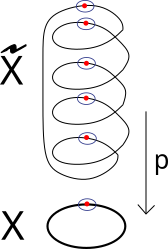
\includegraphics[scale=0.5]{./imagenes/spring.png}
  \end{figure}
  Consideremos a \(x_0 \in [0, 2\pi] /_{0 \sim 2\pi}\) un punto base. El
  homomorfimos inducido para \(p\) corresponde a la función
  \begin{align*}
    p_* : \pi \left( [0, 2\pi] /_{0 \sim 2\pi} , x_0 \right) &\longrightarrow \left( [0, 10\pi] /_{0 \sim 10\pi}, x_0 \right) \\
    [f] &\longmapsto [p \circ f]
  \end{align*}
  Según el diagrama, el claro ver que ambos grupos solo admiten una
  curva no trivial en ellos. Llamaremos
  \begin{gather*}
    [\gamma] \in \pi \left( [0, 10\pi] /_{0 \sim 10\pi}, x_0 \right),\
    \gamma (t) := 10 \pi t \\
    [\alpha] \in \pi \left( [0, 2\pi] /_{0 \sim 2\pi}, x_0 \right), \
    \alpha (t) := 2 \pi t
  \end{gather*}
  a estas. Calculando la imagen de \([\gamma]\) bajo \(p_*\) se obtienen
  las siguiente ecuaciones
  \begin{equation*}
    p_* \left( [\gamma] \right) = [p \circ \gamma]
  \end{equation*}
  donde
  \[
    p \circ \gamma (t) = 10 \pi t \mod 2 \pi = \alpha^5
  \]
  luego, reemplazando en la ecuación anterior
  \begin{equation*}
    p_* \left( [\gamma] \right) = [p \circ \gamma] = [\alpha^5] =
    [\alpha]^5
  \end{equation*}
  Dado que \(p_*\) es un homomorfismo, es claro que \(p_* \left(
  [\gamma]^n \right) = [\alpha]^{5n}\). Conociendo que \(\pi \left(
  [0,2\pi] /_{0 \sim 2\pi} , x_0 \right)\) es \((\mathbb Z, +)\) es claro
  ver que \(p_* \left( \pi \left( [0, 10\pi] , x_0 \right) \right)\) es
  \(5 \mathbb Z \) que es isomorfo (ambos tienen un unico generador) a
  \(\mathbb Z\).
\end{ejemplo}

Una pregunta ha hacerse sobre el teorema \ref{thm:inyec-covering} es si
tenemos esta implicación en sentido contrario, esto es, si todo subgrupo
de \(\pi(X, x_0)\) le corresponde un cubrimiento el cual cumpla esta
relación. La respuesta es afirmativa. La demostración no es nuestro
enfoque, pero se invita a los interesados en revisar el teorema 1.3.6 de
Hatcher \cite{Hatcher}.

Es mas claro la forma de calcular grupos fundamentales usando
cubrimientos. Si estudiamos las imágenes de distintos cubrimientos en el
espacio base, los distintos subgrupos nos darán una idea de
quien debe ser el grupo fundamental del espacio base, pues este debe de
ser compatible con todos los distintos subgrupos generados mediante
cubrimientos. Sin embargo, esta técnica no nos asegura determinar el
grupo del espacio base \(\pi (X, x_0)\) pues nos falta la
sobreyectividad. Buscar condiciones para garantizar esta propiedad es
infructuoso en termino de teoremas. Se adopta otro enfoque en general,
el de estudiar las acciones del grupo \(\pi \left( X, x_0 \right)\)
sobre la fibra \(p^{-1} \left( x_0 \right)\), el cual probaremos que
bajo condiciones sensatas sobre el cubrimiento \(p\) y el espacio
cubrimiento \(\left( \tilde X, \tilde x _0 \right)\), es isomorfo a \(\pi
(X, x_0)\). Estas condiciones están intrínsecamente relacionadas con el
cubrimiento universal

\subsubsection{Cubrimiento universal}
\begin{definicion}[Simplemente conexo]
  Un espacio topológico \(X\) es simplemente conexo si su grupo
  fundamental es trivial.
\end{definicion}
\begin{acotacion}
  Para un espacio simplemente conexo, para cualquier par de arcos
  existe una homotopía entre ellos (la composición de sus dos homotopías
  al arco identidad \(k_{x_0}\)).
\end{acotacion}
Intuitivamente estos espacios son aquellos que no tienen caminos cerrados
triviales. Ejemplo de estos son los distintos \(\Re^n\) para distintos
valores de \(n\).
\begin{definicion}[Cubrimiento universal]
  Sea \(\left( X, x_0 \right)\) un espacio topológico puntuado. Un
  cubrimiento \(p : \left( \tilde X , \tilde x _0 \right) \to \left( X ,
    x _0 \right)\) es llamado cubrimiento universal de \( \left( \tilde
    X , \tilde x _0 \right)\) si \(\left( \tilde X , \tilde x _0
  \right)\) es simplemente conexo.
\end{definicion}
El estudio de los cubrimientos universales esta relacionado con el
comportamiento de una funcion conocida como el levantamiento derivado.
\begin{definicion}[Levantamiento derivado]
  Sea \(p : \tilde X \to X\) un cubrimiento y sea \(x_0 \in X\).
  Escojamos \(\tilde x _0 \in \tilde X\) tal que \(p(\tilde x _0) =
  x_0\). Dado un elemento \([f] \in \pi (X, x_0)\), sea \(\tilde f\) el
  levantamiento (único) de \(f\) a un camino en \(\tilde X\) que
  comienza en \(\tilde x _0\). Se define una función
  \begin{align*}
    \phi : \pi (X, x_0) &\longrightarrow p^{-1} (x_0) \\
    [f] &\longmapsto \tilde f (1)
  \end{align*}
  y denominamos a \(\phi\) como el \textbf{correspondiente levantamiento
  derivado}\footnote{Corresponding lifting path} del cubrimiento \(p\).
\end{definicion}
\begin{acotacion} \label{aco:indep-phi}
  Este mapeo no depende del representante de clase \([f] \in \pi \left(
    X, x_0 \right)\). Para ver esto, notar que tomando a \(f_1 \in [f]
  ,\ f_1 \neq f\) estos están relacionados por una arco-homotopía
  \(H\). Por el teorema \ref{thm:levantamiento-homotopico} de
  levantamiento homotópico, existe una homotopía \(\tilde H\) la cual me
  relaciona los levantamientos \(\tilde f_1 , \tilde f\) de \(f_1 , f\)
  respectivamente. Pero dado el corolario \ref{cor:preservar-arco-hom},
  la homotopía \(\tilde H\) es una arco-homotopía y por tanto
  \[ \tilde f (1) = \tilde H (1, 1) = \tilde H (1, t) = \tilde H (1, 0)
    = f_1 (1) ,\ \forall t \in \{0 \dotsc 1\} \]
  lo que implica que
  \[ \phi ([f]) = \phi ([f_1])\]
\end{acotacion}

Al estudiar los caminos en el espacio base \(\left(X, x_0 \right)\)
cuando estos son levantados al espacio cubrimiento \((\tilde X ,
\tilde x _0 )\), es posible que se transformen caminos con el mismo
punto inicial y final a caminos donde esto no es necesario. Es decir es
posible que ``desenrolle'' los caminos al levantarse. Sin embargo para
cumplir la propiedad de los levantamiento, el punto final de este tiene
que pertenecer al conjunto \(p^{-1} \left( \{x_0\} \right)\), es decir
la fibra de \(x_0\). De hecho podemos enfocarnos puramente en el punto
al que permuta el punto final y podríamos determinar totalmente al arco
en la base al que corresponde cuando el cubrimiento sea universal. Esto
se vera en la siguiente teorema.
\begin{teorema}
  Sea \(p : \tilde X \to X\) un cubrimiento tal que \(p (\tilde x _0) =
  x_0\). Si \(\tilde X\) es arco-conexo entonces el correspondiente
  levantamiento \(\phi : \pi (X, x _0) \to p^{-1} (x_0)\) es
  sobreyectivo. Mas aun, si \(\tilde X\) es simplemente conexo, este es
  biyectivo.
\end{teorema}
\begin{proof}
  Demostración estándar de sobreyectividad en caso de ser \(\tilde X\)
  arco-conexo. Para \(\tilde x _1 \in p^{-1} (x_0)\) arbitrario, existe
  \(\tilde f\) camino entre \(\tilde x _0 \) a \(\tilde x _1\) por
  arco-conexidad. Definimos \(f := p \circ \tilde f\), el cual es un
  camino \(f : I \to X\) que cumple \(\phi ([f]) = \tilde x _1\) por
  definición.

  En caso de ser \(\tilde X\) simplemente-conexo, veremos solo la
  inyectividad. Sean \([f],[g] \in \pi (X, x_0)\) tales que \(\phi([f])
  = \phi([g])\), mostraremos que \([f] = [g]\). Sean \(\tilde f, \tilde
  g : I \to \tilde X\) los levantamientos respectivos que comienzan en
  \(\tilde x _0\). Dado que \(\phi([f]) = \tilde f (1) = \tilde g (1) =
  \phi([g])\) y la simple-conexidad de \(\tilde X\), existe \(\tilde F :
  I \times I \to \tilde X\) homotopía \(\tilde f, \tilde g\). Luego \(p
  \circ \tilde F : I \times I \to X \) es una homotopía entre \(f, g\),
  por tanto \([f] = [g]\)
\end{proof}
% \begin{acotacion}
%   Esta versión del teorema es la mas útil desde el punto de vista del
%   calculo pero no la mas general. Ese enunciado corresponde a estudiar las
%   acciones del grupo \(\pi (X , x_0)\) sobre la fibra. La biyeccion se
%   obtiene de pedir que el cubrimiento sea \emph{regular}, requerimiento
%   que se cumple con pedir simple-conexidad de \((X, x_0)\). Para ver el
%   teorema completo se dirige \cite{Hatcher}[pag. 69]
% \end{acotacion}
Este teorema nos permitirá enfocarnos puramente en la fibra \(p ^{-1}
(x_0)\) para estudiar el grupo fundamental de \((X, x_0)\). Por otro
lado, podemos definir un nuevo grupo el cual va a actuar (en sentido de
grupos) sobre esta fibra al cual denotaremos como grupo de
transformaciones de \emph{deck}\footnote{En español seria transformaciones de
  cartas, pero asi podemos utilizar un nombre usual}.
\begin{definicion}[Grupo de transformaciones de \emph{deck}]
  Para un cubrimiento \(p : \tilde X \to X\), los isomorfismos \(g : \tilde
  X \to \tilde X\) tales que cumplan
  \[ p \circ g = p \]
  son transformaciones de \emph{deck}. El grupo \(G (\tilde X)\) formado
  por estos isomorfismos, la composición como operación forman el grupo
  de transformaciones de \emph{deck} con la función identidad como
  identidad de grupo.
\end{definicion}
Para ver la relación del grupo \(G(\tilde X)\) con la fibra \(p^{-1}
(x_0)\) es necesario generalizar algunos resultados de levantamientos de
caminos (teoremas \ref{thm:lifting-theorem},
\ref{thm:levantamiento-homotopico})

\begin{teorema}
  Sea \(p : (\tilde X , \tilde x_0) \to ( X , x _0 )\) un cubrimiento y
  \(f : (Y , y_0) \to ( X , x _0 )\) una funcion continua con \(Y\)
  arco-conexo y localmente arco-conexo. Entonces un levantamiento
  \(\tilde f : (Y , y_0) \to (\tilde X, \tilde x _0)\) de \(f\) existe
  si y solo si
  \[ f_* \left( \pi (Y, y_0) \right) \subseteq p_* \left( \pi ( \tilde X
      , \tilde x_0 ) \right) \]
\end{teorema}
Que un espacio \(Y\) sea localmente arco-conexo equivale a pedir que
para todo punto \(y \in Y\) y cualquier vecindad \(U_y \subset V\) de
este, posee una sub-vecindad \(V \subseteq U_y\) la cual es arco-conexa.
Procedemos a la demostración.
\begin{proof}
  Se procede en la dirección \((\Rightarrow)\). Por simple definición,
  es fácil ver que \(f_* = p_* \circ \tilde f _*\) lo cual implica
  directamente el resultado.

  Para la dirección \((\Leftarrow)\), sea \(y \in Y\) un punto
  arbitrario. Por arco-conexidad de \(Y\) existe un camino \(\gamma\) en
  \(Y\) tal que \(\gamma (0) = y_0,\ \gamma (1) = y\). Con este podemos
  definir un camino \(f \circ \gamma\) en \(X\) el cual cumple con
  comenzar en \(x_0\). Este ultimo camino tiene un (único) levantamiento
  \(\widetilde {f \circ \gamma}\). Mediante este, definimos una función
  \(\tilde f : (Y, y_0) \to (\tilde X , \tilde x_0)\) por
  \begin{equation} \label{def:f-tilda}
    \tilde f (y) = \phi ([f \circ \gamma]) = f \circ \gamma \, (1)
  \end{equation}
  Esta definición de \(f\) es independiente del camino \(\gamma\)
  escogido entre \(y_0\) e \(y\) por el argumento de independencia de
  representante en \(\phi\) dado en la acotación \ref{aco:indep-phi}.
  Esta acotación depende de la hipótesis \(f_* \left( \pi (Y, y_0) \right)
  \subseteq p_* \left( \pi ( \tilde X , \tilde x_0 ) \right)\) para
  poder levantar homotopías.

  Probaremos la continuidad de \(\tilde f\) en \(y\). Sea \(U \subseteq
  X\) una vecindad de \(f (y)\). Por definición de cubrimiento, existe al
  menos un conjunto \(\tilde U \subseteq \tilde X\) tal que
  \[p \mid_{\tilde U} : \tilde U \to U\]
  es un homeomorfismo. Por otro lado, dada la continuidad de \(f\) y
  por ser \(Y\) localmente arco-conexo se puede elegir una vecindad \(V
  \subseteq Y\) arco-conexa de \(y \in Y\) tal que \(f (V) \subset U\).
  Para todo \(y' \in V\), consideremos los caminos cerrados en \(X\)
  \[ \gamma * \eta * \eta^{-1} * \gamma^{-1} \]
  con \(\gamma\) un camino entre \(y_0 \to y\) y \(\eta\) un camino
  entre \(y \to y'\). Al ver la imagen de este camino bajo \(f\) esta
  corresponde al camino
  \[ (f \circ \gamma) * (f \circ \eta) * (f \circ \eta^{-1}) * (f \circ
    \gamma^{-1}) \]
  en \(X\). Por hipótesis este camino puede ser levantado a
  \(\tilde X\) al camino
  \[ \widetilde{f \circ \gamma} * \widetilde{f \circ \eta} *
    \widetilde{f \circ \eta^{-1}} * \widetilde{f \circ \gamma^{-1}} \]
  En particular es claro que por ser \(p\) un homeomorfismo y \(f (V)
  \subset U\) se tiene que
  \[ \widetilde{f \circ \eta} = p^{-1} \circ f \circ \eta \]
  lo que al juntarse con la ecuación \eqref{def:f-tilda} implica que
  \(\tilde f (V) \subseteq \tilde U\) y en particular \( \tilde f \mid
  _{V} = p^{-1} \circ f \) lo cual es composición de una función
  continua con un homeomorfismo y por tanto continua en \(y\).
\end{proof}

Ahora podemos plantearnos un ejemplo clásico, ver el grupo fundamental
de \(S^1\). Utilizaremos el teorema anterior para proponer un
cubrimiento tal que \(\tilde X\) sea simplemente conexo y que pueda
preservar la estructura de grupo para ser estudiado bajo ese lente.
\begin{teorema} \label{thm:grupo-S1}
  \(\forall x_0 \in S^1,\ \big( \pi (S^1,x_0), * \big)\) es isomorfo a
  \((\mathbb Z, +)\)
\end{teorema}
\begin{proof}
  Dado que \(S^1\) es arco-conexo, basta probar que este teorema es
  cierto para algún \(x_0\) en \(S^1\). Sea \(p : \mathbb R \to S^1,\
  p(t) := (\cos 2 \pi t, \sin 2 \pi t)\) el cual es fue visto anteriormente
  que es un cubrimiento par. Sea \(\tilde x _0 = 0\) y \( p(\tilde x _0) =
  (1,0) =: x_0 \in S^1\). Por ser \(\mathbb R\) simplemente conexo, se
  tiene que el levantamiento correspondiente \(\phi : \pi (S^1, x_0) \to
  p^{-1} (x_0)\) es biyectivo, donde
  \[ p^{-1} (1,0) = \{t \in \mathbb R \mid (\cos 2 \pi t, \sin 2 \pi t)
    = (1, 0) \} = \mathbb Z \]
  Notamos además que de sobre todo \(\mathbb Z\) existe únicamente el
  grupo bajo la adición, este sera nuestro grupo de partida.

  Para probar que es homomorfismo, se toman \([f], [g] \in \pi
  (S^1, x_0)\) arbitrarios y \(\tilde f, \tilde g\) sus correspondientes
  levantamientos tales que \(n := \tilde f (1) = \phi ([f]),\ m :=
  \tilde g (1) = \phi ([g])\). Ahora queremos encontrar quien es el
  levantamiento de \([f] * [g]\), para esto se define el camino
  \begin{align*}
    \tilde{\tilde g} : I &\longrightarrow \mathbb R \\
    s &\longmapsto n + \tilde g (s)
  \end{align*}
  Puesto que \(p(n + x) = p(x)\) por periodicidad, se cumple que
  \[ p \circ \tilde{\tilde g} (x) = p (n + \tilde g (x)) = p (\tilde g
    (x)) = g (x) \]
  Por tanto \(\tilde{\tilde g}\) es el levantamiento de \(g\) para
  \(\tilde x_0 = n\) (en vez de \(\tilde x_0 = 0\)). Luego el producto
  \(\tilde f * \tilde{\tilde g}\) esta bien definido pues \(\tilde f (1)
  = n = \tilde{\tilde g} (0)\) y se afirma que este es el levantamiento
  de \(f * g\) pues por calculo
  \[ p \circ (\tilde f * \tilde{\tilde g}) =
     ((p \circ \tilde f) * (p \circ \tilde{\tilde g})) =
     (f * g)
  \]
  Por ultimo calculamos
  \[ \phi ([f] * [g]) = \tilde{\tilde g} (1) = n + m = \phi ([f]) + \phi
  ([g]) \]
  Por lo que \(\phi\) es un homomorfismo de grupos.
\end{proof}

\begin{ejemplo}[Cubrimiento \(p_n : S^1 \to S^1\)]
Para testear la intuición
de que el espacio cubrimiento refleja en el caso común un subgrupo del
espacio topológico, tomemos el caso
\begin{align*}
  p_n : S^1 &\longrightarrow S^1 \\
  z &\longmapsto z^n
\end{align*}
Para este, nuestro conjunto \(p^{-1} (x_0)\), con \(x_0 = (1,0)\) se
obtiene mediante la reducción
\begin{align*}
  p^{-1} (1,0)
    &= \{ z \in S^1 \mid z^n = (1,0)\} \\
    &= \{z \in S^1 \mid (\cos 2 \pi n t, \sin 2 \pi n t) = (1,0) :
           t \in [0,1] \} \\
    &= \{(\cos 2 \pi t, \sin 2 \pi t) \in S^1 \mid
           t \in \{0, \frac 1 n , \dotsc , \frac {n-1} n \} \}
\end{align*}
\[ \therefore p^{-1}(1,0) \simeq \mathbb Z / n \mathbb Z \]
Además bajo el mismo tratamiento utilizado anteriormente en \(\pi (S^1,
x_0) = \mathbb Z\) para \(\phi\), este es un homo-morfismo. Esto muestra
que la elección de \(p\) afecta que subgrupo de \(\pi (S^1, x_0)\) estudiaremos.
\begin{teorema}
  Sea \(p : \tilde X _1 \to X_1,\ p' : \tilde X _2 \to X_2 \) dos
  cubrimientos pares, entonces
  \[ p_1 \times p_2 : \tilde X _1 \times \tilde X _2 \to X_1 \times X_2 \]
  Es un cubrimiento par.
\end{teorema}
\begin{proof}
  Para todo \(x_1 \in X_1,\ x_2 \in X_2\), existen \(U_1, U_2\)
  vecindades pares respectivamente tales que son cubiertas por \(p_1,
  p_2\). Denotemos a \(\{V_\alpha^{(1)}\}, \{V_\beta^{(2)}\}\) familias
  de conjuntos tales que
  \[
    \begin{matrix}
      \bigcup_{\alpha} V_\alpha^{(1)} = p_1^{-1} (U_1) &
      \bigcup_{\alpha} V_\alpha^{(2)} = p_2^{-1} (U_2)
    \end{matrix}
  \]
  \[ \bigcup_{\alpha, \beta} V_\alpha^{(1)} \times V_\beta^{(2)} = (p_1
    \times p_2)^{-1} (U_1 \times U_2)\]
  Donde la restricción a un \(V_{\bar{\alpha}}^{(1)} \times
  V_{\bar{\beta}}^{(2)}\) arbitrario en \(p_1 \times p_2\) obtiene un
  homeomorfismo en virtud de las componentes.
\end{proof}
\end{ejemplo}

Esto es una extensión del resultado que ya conocíamos sobre el functor
entre \(\mathbf{HoTop}_{*}\) y \(\mathbf{Grp}\) en cuanto a preservación
del producto. Esto no dice que el ``calculo'' de grupos fundamentales
también puede derivarse del conocimiento del productor de cubrimientos
pares.

\begin{ejemplo}[Toro en \(R^4\).]
Dado que podemos caracterizar al
toro \(T^1\) como \(S^1 \times S^1\), el teorema anterior nos dice que
\((\pi (T^1, b), *) = (\pi (S^1, b) \times \pi (S^1, b), *) = (\mathbb Z
\times \mathbb Z, +) \)
\end{ejemplo}